\chapter{Localization Technologies}
\label{cha:relatedwork}

\section{Related Work}

Before we started our project we did research on related work regarding applied indoor navigation and positioning techniques applied on mobile devices. Most of them rely on calculating Received Signal Strength Indicator (RSSI) triangulation and/or Bluetooth BLE Beacon techniques or Wi-Fi Based Fingerprinting. The latter is a core idea of an indoor navigation system developed by \cite{ChaSo2012}. They combine two methods in order to calculate a precise position. At first they use matching of prerecorded received signal strength from nearby access points. This method is called \enquote{fingerprint matching}. The data is combined with a distance-based trilateration approach with at least three known access point coordinates which are also detected on the device. By this combination of both methods they received a high accuracy of the user position in an indoor environment.

\cite{Feldmann12} implemented an indoor Bluetooth-based positioning system on Bluetooth-capable devices as a PDA, which is comparable to the smartphones of today. They calculated range estimations based on approximations of relations between RSSI and distance between sender and receiver. The location estimation was also calculated via triangulation method.

Apple Inc. presented on WWDC2015 new features of there well known Core Location Frameworks providing Indoor positions and Floor information \cite{wwdc15}. The closed beta is restricted by access to developers that are registered on Apples Indoor Program Maps Connect. Although Apple does not publish its algorithms, as stated on WWDC2015 by Apple Software Engineer Vitali Lovich the Core Location Frameworks also takes advantage of indoor WiFi signals in combination with motion and altitude sensors in order to provide the users with accurate position information as latitude and longitude.

In 2013 Apple also developed the iBeacon protocol which is a Bluetooth Low Energy (BLE) communication standard supported by iOS and Android devices \cite{iBeacon}. The iBeacon protocol opened the door for new Beacon technologies in order to improve indoor navigation on mobile devices. The standard is incorporated by Estimote Inc. with Estimote Beacons. This indoor technique has successfully been installed in museums such as the Metropolitan Museum of Art project called: MediaLab Beacon Art Walk \cite{MOArt15}. However, this project aimed to provide additional location information to the visitors rather than providing indoor positions. Next to the battery issues also faced in the MediaLab Project, Beacons having difficulties  in cases of many people covering the clear line of sight to a device, makes actual retrieving of Latitude/Longitude coordinates in a room more difficult. Next to this, installed beacons made  temporarily maintaining of Beacons mandatory, since one missing Beacon could prevent successful indoor navigation in a calibrated system.

The Cisco MSE approach moves the calculation of a position away from a device \cite{oreilly11}. Correctly installed Cisco MSE determines the location of any wireless device in a Building. The access points listen for Wi-Fi signals of devices and estimate its position also via trilateration. This solution can be seen at the American Museum of Natural History \cite{AMNH15}.

The Cisco MSE determines the location of any wireless device in a specific building. One approach is to make the building do the work instead of the device. Some WiFi installations, such as the Cisco MSE, can determine the location of any wireless device in the building. The access points themselves listen for the WiFi signals created by your phone, then estimate its position via trilateration. This solution has been deployed successfully at a few locations as mobile application for visitors, like the Explorer App  at the American Museum of Natural History.


\vspace{0.5cm}

\section{Short range localization techniques}
\label{short_range_localization_techniques}
Different localization techniques are presented and compared in book~\cite{brimicombe2009location}. For purpose of this project, we were interested mostly in short range positioning technologies. Short range positioning technologies cover small areas and are frequently employed for positioning in indoor environments. Most popular technologies are WiFi and Bluetooth, which are most commonly used to determine proximity location of mobile device connected to network. Other available technologies are Radio Frequency Identification (RDIF), Ultra Wide Band Positioning, ultrasonic positioning, infrared positioning, camera-assisted and sensor-assisted positioning. We focused our research on Wi-Fi and Bluetooth as those were the technologies provided for us by our supervisors.

\subsection{WiFi based positioning}
The basic principle of using WiFi for indoor positioning is measuring strength of signals received at two or more access points. The signals used for positioning are called beacon frames and are primarily intended for announcing the presence of a wireless LAN. There are two ways of transmitting these signals for positioning, up-link, when beacon frames are generated by mobile device and down-link, where beacon frames are generated by access points.

Actual positioning can be done in three ways. The simplest method is determining position of mobile device from position of the access point with the strongest signal, which is the closest to the mobile device. In this case a data linking access points and their locations is needed. The second method uses signal strength data from multiple access points to calculate the position of mobile device. This method provides more accurate position data. Third method uses fingerprinting approach, in which position is determined by matching signal data on mobile device against set of precollected data on signal strengths across the area. This approach offer the best results, but it requires initial measurement of the area before position tracking can take place.

WiFi based positioning only works in areas with good wireless network coverage. It is most commonly used in closed spaces such as offices, airports, cafes, shopping markets, hotels etc. It can also be used for outdoor positioning, usually in dense populated urban areas.

In general, WiFi positioning provides a proximity location instead of more specific coordinates. For example, it may provide information, in which building, floor and room mobile device is located. When using WiFi positioning there is no need for additional infrastructure, except for existing WiFi network and positioning server with database of all available access point along with their positions.

\subsection{Bluetooth based positioning}
Various solutions have been developed using Bluetooth for short range positioning. Bluetooth enabled devices are able to transmit signals containing information such as device identity and profile. When mobile device is in short range of device transmitting its location it can pick up such signals and use them for positioning. Signals can also be processed to determine the position of device, especially in case when mobile device can receive multiple signals from different devices. Position data can be exchanged between mobile devices using ad-hoc Bluetooth networks or with the location server in the network.

The signal strength decreases logarithmically with distance. This property can be used for calculating position. One method of positioning device is to triangulate data from different devices. This method offers higher accuracy than just detecting the closest device in range.

Bluetooth positioning can be deployed rapidly with easy maintenance and low cost. It can be used in applications where approximate positioning is sufficient.

Different implementations of WiFi and Bluetooth based localization technologies are described in more detain in following sections.


\vspace{0.5cm}

\section{Bluetooth Low Energy}

Multiple solutions are based on the already mentioned Bluetooth Low Energy (BLE) standard. To understand the reasons for this standard in comparison to classic Bluetooth better, we had \enquote{Bluetooth Low Energy - The Developer's Handbook} by Robin Heydon, published with Prentice Hall in 2012, available \cite{heydon2012bluetooth}. In the following we try to point out some specifics of BLE taken from the just mentioned book.

Heydon starts by stating that although BLE has obvious connections to its parents, the classic Bluetooth standards, \enquote{Bluetooth low energy should be considered a different technology, [...].} (ibid., p. 3). This is a consequence derived from the different design goals the developers had when they set out to standardize what would become Bluetooth Low Energy. The new standard is not a performance upgrade but by design focused on totally different obstacles. \enquote{When the low energy work started, the goal was to create the lowest-power short-range wireless technology possible.} (ibid., p. 7). This resulted in following goals: worldwide operation, low cost, robust, short range, low power (ibid., p. 7).

Bluetooth Low Energy does not try to be yet another bandwidth upgrade for Bluetooth but rather a step towards extremely low power consumption as well as being very cheap. This latter directive makes it possible for Bluetooth Low Energy to be deployed in high volumes. In order to achieve this, Bluetooth Low Energy makes use of following three design points:

\begin{itemize}
    \item \textbf{Operation on 2.4 GHz ISM band}. It's an overused band and has bad characteristics as it is heavily absorbed by water which is the biggest part of the human body. But also no license fees are taken to operate on this band and therefore, \enquote{choosing to use the ISM band lowers the cost} (ibid., p. 5).
    \item \textbf{Intellectual property (IP) license for usage}. Basically, the Bluetooth Special Interest Group (SIG) is claimed to be cheaper than other SIGs. Licenses are given under a FRAND policy which stands for \enquote{Fair, Reasonable, and Non-Discriminatory} (ibid., p. 5).
    \item \textbf{Low power consumption}. Aiming at low power consumption overall reduces the costs of accompanying services and material costs.
\end{itemize}

This results in transmission speeds that are way below the ones of the classic Bluetooth versions, even lower than the speed of some very early standard versions of Bluetooth. Following table reviews the speeds of the existing Bluetooth variants (ibid., table 1-1, p. 4):

\begin{center}

    \begin{tabular}{ c | c }
        \textbf{Bluetooth standard} &   \textbf{Maximum bandwidth} \\
        \hline
        v1.1                        &   1 MBps \\
        v2.0                        &   3 MBps \\
        v3.0                        &   54 MBps \\
        v4.0 (BLE)                  &   0.3 MBps
    \end{tabular}

\end{center}

Therefore BLE is not tailored on the use cases classic Bluetooth tackles, \enquote{[...] because single mode Bluetooth low energy does not support audio for headsets and stereo music or high data rates for file transfers.} (ibid., p. 6). It is to be used in situations where extremely low power consumption is needed while at the same time the amount of data transferred is kept low.

To survive in the congested frequency band it operates on, Bluetooth Low Energy uses adaptive frequency hopping. A technique that detects sources of interference, helps to avoid them in the future and quickly recovers from dropped packages. \enquote{It is this robustness that is absolutely key to the success of any wireless technology in the most congested radio spectrum available.} (ibid., p. 8).

Another consideration is the distance BLE is able to cover and Heydon concludes that \enquote{[s]hort range means that Bluetooth low energy should be a \textbf{person area network}} (ibid., p. 8).


\vspace{0.5cm}

\section{Estimote Beacons}

Estimote Beacons and Stickers are wireless sensors that can be attached to any location or object, embodying a wireless sensor network. The Beacons consists of a 32-bit ARM Cortex CPUs, equipped with an accelerator, temperature sensor and a 2.4 Ghz radio. Using Smart Bluetooth 4.0.(Bluetooth low energy), the beacons send out signals with a range of up to 70 meters (Beacons) and 15 meters (Stickers). Though the signals are often distracted under real world conditions, a range of about 40-50 and (Beacons) can be suspected. The battery can as stated by \cite{Estimote} last more than 3 years on default settings on a single CR2477 battery.

Estimote beacons are working with the Apple iBeacon protocol as well as the Eddystone  open beacon format introduced by Google. These protocols working on top of the BLE technology standard are implemented in all smartphones devices enabling them to support new technologies like Apple Watch or Fitness trackers.

Using the Estimote SDK \cite{Estimote} mobile applications are enabled to receive and understand BLE Estimote signals in order to calculate the proximity to nearby locations and objects. The beacons specifics provide information about their type, ownership and approximate locations, temperature or motions.

By the detecting a beacon signal a phone can estimate the distance by measuring the received signal strength \cite{Estimote}. Since Bluetooth Low Energy does not need any pairing process between sender and receiver, the phone can constantly process new signals. this opens the doors for new technologic opportunities as indoor location/ indoor positioning.


\subsection{iBeacon Protocol}

The iBeacon protocol is a Bluetooth low energy communication protocol developed by Apple Inc. in 2013 and was introduced in iOS7 for indoor navigation. The protocol is supported by iOS7 devices as well as Android from version 4.3 up. The signal which is sent by a beacon is called advertisement.

These advertisements provides a so called iBeacon identifier, that is is 20 bytes long and divided into three sections:

\begin{itemize}
    \item UUID (16 bytes)
    \item major number (2 bytes)
    \item minor number (2 bytes)
\end{itemize}

These values provided by the advertisement can be modified according to own wishes.
The hierarchical configuration of these values provides identifying information about the beacon. While the UUID can be distinguished to a corporation, major and minor values can be used to distinguish between regions and sub-regions of a corporation.


\subsection{Region Monitoring}

Region monitoring triggers actions on the device on entering or exiting a beacon defined regions range. This works in depending the devices capabilities while an app is in foreground background or suspended. An app is limited to 20 regions being monitored. However by using a single UUID in multiple locations, a device can monitor many physical locations simultaneously \cite{iBeacon}.


\subsection{Ranging}

Ranging however triggers actions on the devise based on the proximity to a beacon.
The iBeacon protocol applies filters to the accuracy of a advertisement of one beacon. The filtered estimation regarding the proximity to a beacon is indicated using one of four proximity states.

\begin{itemize}

    \item \textbf{Immediate}\\
    The Immediate proximity state represents a high level of confidence, that the device is physically very close to the beacon. This is in example holding the smartphone directly on to of a beacon.
    \item \textbf{Near}\\
    The Near proximity state indicates a proximity of round about 1-3 meters, if there are no obstructions between the device and the beacon which might cause distractions of the beacon.
    \item \textbf{Far}\\
    The Far proximity state indicates a detected beacon without much confidence in the accuracy that is to low to determine whether it is Near or Immediate. The Far proximity state relies on the accuracy property to determine the potential proximity to the beacon.
    \item \textbf{Unknown}\\
    The Unknown proximity state indicates a state where beacons are can not be determined. This my happen if the ranging has just begun or that the accuracy level is insufficient for measurements to determine a state that is either Far, Near or Immediate.
\end{itemize}

\subsection{Estimote Beacon Drawbacks}

For the implementation of Estimote Indoor Navigation for the project we decided to use Monitoring on the devices in order to detect the beacons, specifying a certain region. However, the devices still take at least about 30 seconds to recognize the fact that a beacon is out of range. This is a  built-in and non adjustable delay in order to prevent \enquote{false} exit events.\cite{Estimote} This is a major drawback regarding a use-case of the project, that a user might pass multiple beacons of a location and constantly update new locations without the need to stop at each beacon.

This is solved by in additional applied ranging of all beacons that are monitored in order to process the \enquote{nearest} beacon as a users location. The devices report then the beacons in an order that is best guess of their proximity regarding issues of signal attenuation. This order however may still not be correct \cite{iBeacon}.


\vspace{0.5cm}

\section{Apple Core Location Framework}

As firstly presented on WWDC2015 \cite{wwdc15}  Apple presented new functionalities to the already existing Core Location Framework which is the major Framework on iOS devices for location service \cite{CLlocation}. This Framework takes the user in charge of whether the app can use locations services on the device or not.

The Core Location Framework uses Cellular data to provide a proximity in which area in a city a user is. Additionally it uses GPS based on Satellite signals to improve the position of the user as well as surrounding WiFi signals.

As soon as the user enters an indoor venue, the iOS system turns down GPS and Cellular sensors and enlightens Motion and WiFi sensors.
These sensors are used in combination with the remaining GPS signals, coming through the windows to locate the user indoors. The Motion sensor hereby gives information to the system that a person is moving and how fast the user is moving, while wi-fi signals are feeded to the CLLocation Framework to calculate the exact position.

Apple also added the altitude and floor attributes to the CLLocation Framework in order to provide the user with the correct floor attributes \cite{CLlocation}.

For the Project the new CLLocation Framework was used to show the users positon in the Mensa. After the first indoor tests in the Mensa revealed precise positioning of a user indoors. However the Framework also revealed large susceptibility in areas where the WiFi signal was apparently weak. i.e. in the upper left corner of the Mensa which is surrounded by walls that are affecting the router WiFi signals.

The Frameworks started in an early beta when this project started and is constantly improved. To enable the full abilities of CLLocation Framework indoors, the venue needs to be registered and enabled by apple, using Maps Connect program \cite{MapsConnect} in order to unlock CLLocation Frameworks full potential.

Regarding this project we tested the indoor navigation framework to see if its accuracy is already sufficient for our use case in the Mensa. As shown in  ~\ref{fig:cllocationframework1} and ~\ref{fig:cllocationframework2} The user location is shown precisely on the indoor floorplan. The accuracy as shown in ~\ref{fig:cllocationframework1} started with a large circle but constantly improved while moving through the building. We also accounted situations in which the framework lost precision dramatically as we moved to the upper left corner of the Mensa which is surrounded by walls. However the provided coordinates of the shared position of the user to the system was still accurate enough in order to find a friend.

We decided to use this technology, since it is the only solution for this project in order to show the user position on the floors without any additional installations into the environment of the Mensa, out of the box and without any additional user interaction.

\begin{figure}
\centering
\begin{minipage}{.5\textwidth}
  \centering
  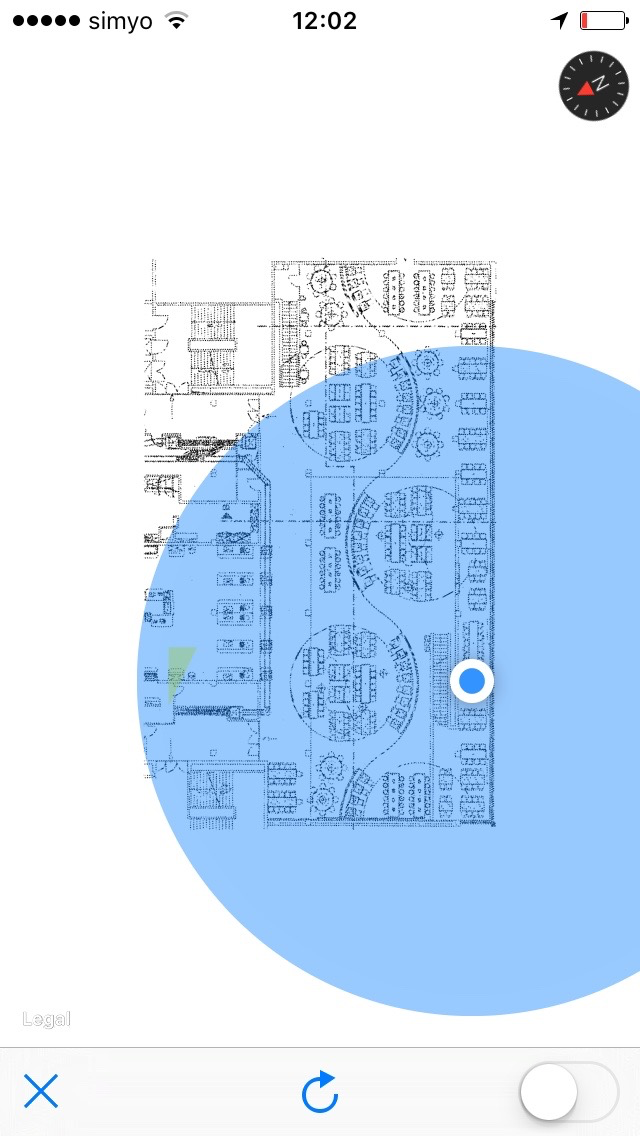
\includegraphics[width=.5\linewidth]{cllocationframework1}
  \captionof{figure}{Indoor Position on start}
  \label{fig:cllocationframework1}
\end{minipage}%
\begin{minipage}{.5\textwidth}
  \centering
  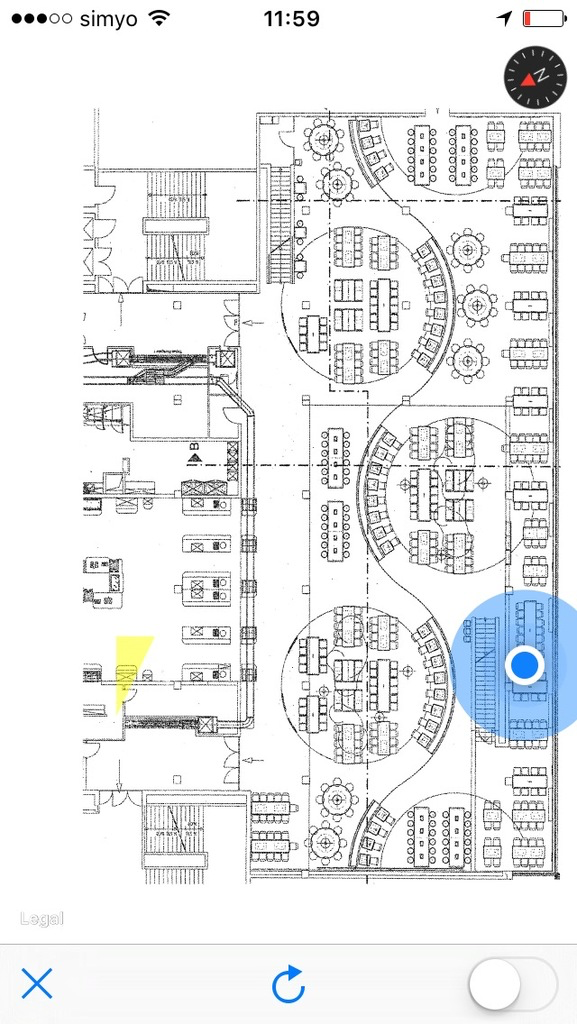
\includegraphics[width=.5\linewidth]{cllocationframework2}
  \captionof{figure}{Accuracy drastically improved after a couple of seconds }
  \label{fig:cllocationframework2}
\end{minipage}
\end{figure}


\vspace{0.5cm}

\section{CISCO MSE API Wrapper Tests}

In order to determine whether the CISCO MSE API wrapper provided by tubIT would be sufficient for the project's requirements we were asked to perform tests on it. Especially it was asked for details on how the API worked where, so what values could be retrieved via the API wrapper in which locations on campus and how precise the values would turn out to be.

Concerning use cases our project was focused on the Mensa and the library, therefore we initially planned to be conducting tests in only these two locations. As the provided wrapper around the CISCO MSE API we had access to delivered back one short, simple XML line we decided to invest some time into developing a small tool which routinely queried the API for it's current status and saved the result into an easily readable JSON file for later investigation. The source code of the developed tool you can find in appendix \ref{appendix:cisco-mse-api-test}.

\begin{center}
    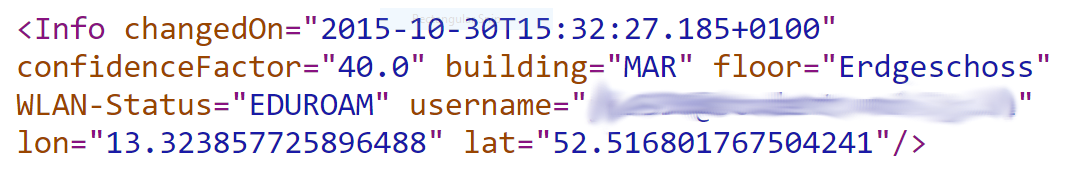
\includegraphics[width=\textwidth]{cisco-mse-api-response}\\
    What the CISCO MSE API wrapper response looks like.
\end{center}

It was planned to be conducting the tests on one day in the Mensa and on another day in the library. On the first day we started around noon and ran the test tool on one of our notebooks connected to university WiFi, \enquote{eduroam}. We started in the south-western corner near the windows, walked towards the south-eastern corner, went to the stairs in the northern part and upstairs and again at the window front to the south-western corner on the first floor. As it turned out, the results we got back were definitely not what we had hoped for, most importantly because longitude and latitude of the requesting user were missing completely. The following listing shows the first ten results logged in two second periods from the API wrapper:

\begin{lstlisting}
{
    "signal": [
        {"timestamp": 1445344391, "latitude": "0.000000000000000", "longitude": "0.000000000000000", "building": "Mensa", "floor": "Mensa 1. OG"},
        {"timestamp": 1445344393, "latitude": "0.000000000000000", "longitude": "0.000000000000000", "building": "Mensa", "floor": "Mensa 1. OG"},
        {"timestamp": 1445344395, "latitude": "0.000000000000000", "longitude": "0.000000000000000", "building": "Mensa", "floor": "Mensa 1. OG"},
        {"timestamp": 1445344397, "latitude": "0.000000000000000", "longitude": "0.000000000000000", "building": "Mensa", "floor": "Mensa 1. OG"},
        {"timestamp": 1445344399, "latitude": "0.000000000000000", "longitude": "0.000000000000000", "building": "Mensa", "floor": "Mensa 1. OG"},
        {"timestamp": 1445344401, "latitude": "0.000000000000000", "longitude": "0.000000000000000", "building": "Mensa", "floor": "Mensa 1. OG"},
        {"timestamp": 1445344404, "latitude": "0.000000000000000", "longitude": "0.000000000000000", "building": "Mensa", "floor": "Mensa 1. OG"},
        {"timestamp": 1445344406, "latitude": "0.000000000000000", "longitude": "0.000000000000000", "building": "Mensa", "floor": "Mensa 1. OG"},
        {"timestamp": 1445344408, "latitude": "0.000000000000000", "longitude": "0.000000000000000", "building": "Mensa", "floor": "Mensa 1. OG"},
        {"timestamp": 1445344410, "latitude": "0.000000000000000", "longitude": "0.000000000000000", "building": "Mensa", "floor": "Mensa 1. OG"},
        ...
    ]
}
\end{lstlisting}

Clearly it can be observed that the longitude and latitude values are unusable. Another take away was that the floor change during our test did not reflect into our captured results. Therefore we decided to directly test the library for comparable results. Inside the library, we started on ground floor and went upstairs in \enquote{circles} through the different levels. From the fourth floor we went back down straight forward. During that second test ten of the first fifteen responses from the API looked like:

\begin{lstlisting}
{
    "signal": [
        {"timestamp": 1445345843, "latitude": "0.000000000000000", "longitude": "0.000000000000000", "building": "BIB", "floor": "Erdgeschoss"},
        {"timestamp": 1445345845, "latitude": "0.000000000000000", "longitude": "0.000000000000000", "building": "BIB", "floor": "Erdgeschoss"},
        {"timestamp": 1445345848, "latitude": "0.000000000000000", "longitude": "0.000000000000000", "building": "BIB", "floor": "Erdgeschoss"},
        {"timestamp": 1445345850, "latitude": "0.000000000000000", "longitude": "0.000000000000000", "building": "BIB", "floor": "Erdgeschoss"},
        {"timestamp": 1445345852, "latitude": "0.000000000000000", "longitude": "0.000000000000000", "building": "BIB", "floor": "Erdgeschoss"},
        {"timestamp": 1445345854, "latitude": "0.000000000000000", "longitude": "0.000000000000000", "building": "BIB", "floor": "Erdgeschoss"},
        ...
        {"timestamp": 1445345870, "latitude": "0.000000000000000", "longitude": "0.000000000000000", "building": "BIB", "floor": "1. Obergeschoss"},
        {"timestamp": 1445345872, "latitude": "0.000000000000000", "longitude": "0.000000000000000", "building": "BIB", "floor": "1. Obergeschoss"},
        {"timestamp": 1445345874, "latitude": "0.000000000000000", "longitude": "0.000000000000000", "building": "BIB", "floor": "1. Obergeschoss"},
        {"timestamp": 1445345876, "latitude": "0.000000000000000", "longitude": "0.000000000000000", "building": "BIB", "floor": "1. Obergeschoss"},
        ...
    ]
}
\end{lstlisting}

First, longitude and latitude were again unusable. This time though the floor information worked quite reliably and indicated very fast on which floor we currently measured. After that we were wondering whether eventually we would get back longitude and latitude values anywhere on campus and decided to give it one last try by taking one more measurement in the MAR building (Marchstraße).

One more measurement turned into three as during the first two attempts we got sudden disconnects and therefore unusable results. We walked the whole foyer from north to south side and somewhere near the entrance we suspect the wireless signal got bad and our notebook conducting the tests disconnected. In the third try though we finally were able to get back usable results, in which chosen ten results logged looked like this:

\begin{lstlisting}
{
    "signal": [
        {"timestamp": 1445350550, "latitude": "52.516903688639005", "longitude": "13.323958376544699", "building": "MAR", "floor": "Erdgeschoss"},
        {"timestamp": 1445350552, "latitude": "52.516903688639005", "longitude": "13.323958376544699", "building": "MAR", "floor": "Erdgeschoss"},
        {"timestamp": 1445350554, "latitude": "52.516903688639005", "longitude": "13.323958376544699", "building": "MAR", "floor": "Erdgeschoss"},
        {"timestamp": 1445350557, "latitude": "52.516903688639005", "longitude": "13.323958376544699", "building": "MAR", "floor": "Erdgeschoss"},
        ...
        {"timestamp": 1445350686, "latitude": "52.516864921942748", "longitude": "13.323953890659670", "building": "MAR", "floor": "Erdgeschoss"},
        {"timestamp": 1445350688, "latitude": "52.516864921942748", "longitude": "13.323953890659670", "building": "MAR", "floor": "Erdgeschoss"},
        {"timestamp": 1445350690, "latitude": "52.516864921942748", "longitude": "13.323953890659670", "building": "MAR", "floor": "Erdgeschoss"},
        ...
        {"timestamp": 1445350845, "latitude": "52.516402095317481", "longitude": "13.323531401046099", "building": "MAR", "floor": "Erdgeschoss"},
        {"timestamp": 1445350847, "latitude": "52.516402095317481", "longitude": "13.323531401046099", "building": "MAR", "floor": "Erdgeschoss"},
        {"timestamp": 1445350849, "latitude": "52.516402095317481", "longitude": "13.323531401046099", "building": "MAR", "floor": "Erdgeschoss"},
        ...
    ]
}
\end{lstlisting}

Finally we received some longitude and latitude values. Unfortunately the three different pairs of longitude and latitude above were the only ones we could observe during the whole walk from north end to south end of the foyer, thus still rather unusable values.

In the end, our conclusion at that point in the project progress was to use the CISCO MSE API wrapper provided by the tubIT in order to retrieve the rough position of a user. This means the building and floor the request originated from. We recommended back to our supervisors not to use this API for receiving longitude and latitude as these values were either quite imprecise or not available at all. The full result files of all our three measurements can be found at \cite{ioslINavGitHub}.


\vspace{0.5cm}

\section{Evaluation of Available Technologies}
As mentioned in \ref{short_range_localization_techniques}, WiFi and Bluetooth based positioning technologies are the most suitable and most widely used for indoor positioning. With technology development such as Bluetooth Low Energy and different wrapper implementations such as CISCO MSE API those two technologies became even more important players in indoor navigation. Review of related work confirms this statement, as majority of related work use those two technologies.

This research and related work presented the basics for our decision on which technologies to use. Our decision was also biased by the infrastructure and equipment we had at our disposal. tubIT provides the wrapper for CISCO MSE API in the university campus and because WiFi based localization techniques are widely used for indoor positioning, we decided to give it a try. It turned out to be quite ineffective at retrieving exact coordinates of user. However, since it provides quality information about building name and floor all over the university campus, we decided to include it in our project as least accurate positioning technique. We also had 3 Estimote Beacons and 6 Stickers at our disposal. Since Bluetooth positioning techniques are widely used for indoor positioning, we considered Estimote Beacons and Stickers as possible localization technique for our project. Their usage of Bluetooth Low Energy which provides low cost, robustness and low power usage represented big plus in their favor. The biggest plus was their support for iBeacon protocol which makes them compatible with all modern mobile devices. All those factors supported our decision to use Estimote Beacons and Stickers in our project.

Since we planned to implement both Android and iOS client, we decided to use Apple Core Location Framework on iOS devices. Decision was supported by the fact that this new technology provides quality indoor location information using wildly deployed and available technology WiFi and that it may play an important role as indoor navigation technology in future releases of iOS operating system.